\documentclass[a4paper, 12pt, reqno]{amsart}

\usepackage{amssymb}
\usepackage{amsfonts}
\numberwithin{equation}{section}
\usepackage[margin=1in]{geometry}
\usepackage[english]{babel}
\usepackage[colorlinks, pdftitle={Actuarial Mathematics Homework 1 and 2},
    pdfauthor={Moritz M. Konarski}]{hyperref}
\usepackage{enumitem}
\usepackage{graphicx}

\title{Actuarial Mathematics Homework 1 and 2}
\author{Moritz M. Konarski}
\date{\today}

\begin{document}

\maketitle

\section*{Homework 1}

\subsection*{1--1}

\begin{enumerate}[label=(\alph*)]
    \item 20,720.00000
    \item 22,216.24052
    \item 14,202.52055
    \item 16,497.81725
\end{enumerate}

\subsection*{1--2}

\begin{enumerate}[label=(\alph*)]
    \item 23,590.81417
    \item 22,114.94444
    \item 24,290.01969
\end{enumerate}

\subsection*{1--3}

It is not true. It is only true for $n \ge 2$.

\begin{equation}\nonumber
    \begin{aligned}
        i_1 &= 2 \\
        i_2 &= \frac{4}{3}  \\
        \vdots
    \end{aligned}
\end{equation}

\subsection*{1--4}

\begin{enumerate}[label=(\alph*)]
    \item $a(0) = \sqrt{1}$; $a(1) = \sqrt{1 + (i^2 +2i)} = 
        \sqrt{(i + 1)^2} = 1+i$
    \item square roots are continuous and always increasing
    \item $a(1) = \sqrt{i^2 + 2i + 1}$, $a(0.5) = \sqrt{0.25i^2 + 0.5i + 1}$,
        so $a(0.5) < a(1)$ \\
        $a(2) = \sqrt{4i^2 + 8i + 1}$, here $a(1) < a(2)$
    \item for $t=1$ both equations are equal, $(1+i)^t$ grows quicker, so for
        all $t>1$ this holds
\end{enumerate}

\subsection*{1--5}

\begin{enumerate}[label=(\alph*)]
    \item for an exponential function $a(0)=1$, $i_n$ can be found
        \begin{equation}\nonumber
            \begin{aligned}
                i_n &= \frac{a(n) - a(n-1)}{a(n-1)}                 \\
                    &= \frac{(1+i)^n - (1+i)^{n-1}}{(1+i)^{n-1}}    \\
                    &= ((1+i)^n - (1+i)^{n-1}) \cdot (1+i)^{-n+1}   \\
                    &= (1+i)^n \cdot (1+i)^{-n+1} 
                        - (1+i)^{n-1} \cdot (1+i)^{-n+1}            \\
                    &= (1+i)^{1} - (1+i)^{0}                        \\
                    &= 1+i-1                                        \\
                i_n &= i \qed
            \end{aligned}
        \end{equation}
    \item yes, as the above proof works for all $n$
\end{enumerate}

\subsection*{1--13}

\begin{enumerate}[label=(\alph*)]
    \item 681.472
    \item 0.13636
    \item 681.479 -- yes it is the same, the lost precision in (b) is the
        reason for the slight difference
\end{enumerate}

\subsection*{1--14}

\begin{enumerate}[label=(\alph*)]
    \item 7,092.8357
    \item 6,501,65722
    \item we learned that $d < i$ for one problem. Here they are equal, meaning
        that if we convert $d=0.12$ to $i$ it will be larger. $d$ here is
        equivalent to $i=0.1363$ which explains why they numbers are different.
        Higher compound interest rates mean that value increases faster but if
        one goes back in time they decrease faster too. That's why (b) is
        lower
\end{enumerate}

\subsection*{1--15}

\begin{enumerate}[label=(\alph*)]
    \item See \textsc{Figure 1.}
        \begin{figure}[h]
            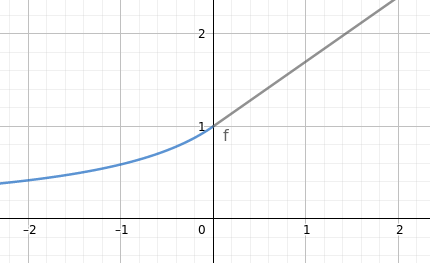
\includegraphics[width=0.7\textwidth]{../graph}
            \caption{Graph of $a(t)$ for simple interest, $i=0.7$}
        \end{figure}
    \item $1-it$ is not correct because it does not follow from the formula for
        accumulation.
\end{enumerate}

\subsection*{1--16}

\begin{enumerate}[label=(\alph*)]
    \item we proved earlier that $i_n$ is constant for compound interest, and
        we can express $d_n$ in terms of $i_n$
        \begin{equation}\nonumber
            d = \frac{i}{1+i}
        \end{equation}
\end{enumerate}

\subsection*{1--17}

\begin{enumerate}[label=(\alph*)]
    \item \begin{equation}\nonumber
            \begin{aligned}
                d &= i \cdot v              \\
                  &= i \cdot \frac{1}{1+i}  \\
                d &= \frac{i}{1+i} \qed
            \end{aligned}
        \end{equation}
    \item \begin{equation}\nonumber
            \begin{aligned}
                d &= 1 - v              \\
                  &= 1 - \frac{1}{1+i}  \\
                  &= \frac{1+i}{1+i} - \frac{1}{1+i}  \\
                  &= \frac{1+i-1}{1+i}  \\
                d &= \frac{i}{1+i} \qed
            \end{aligned}
        \end{equation}
    \item \begin{equation}\nonumber
            \begin{aligned}
                i-d &= i \cdot d              \\
                \frac{d}{1-d} - d &= \frac{d}{1-d} \cdot d  \\
                \frac{d}{1-d} - \frac{(1-d)d}{1-d} &= \frac{d^2}{1-d} \\
                \frac{d-d + d^2}{1-d} &= \frac{d^2}{1-d} \\
                \frac{d^2}{1-d} &= \frac{d^2}{1-d} \qed
            \end{aligned}
        \end{equation}
    \item \begin{equation}\nonumber
            \begin{aligned}
                \frac{1}{d} - \frac{1}{i} &= 1   \\
                \frac{1}{d} - \frac{1}{\frac{d}{1-d}} &= 1   \\
                \frac{1}{d} - \frac{1-d}{d} &= 1   \\
                \frac{1-1+d}{d} &= 1   \\
                \frac{d}{d} &= 1   \qed
            \end{aligned}
        \end{equation}
    \item \begin{equation}\nonumber
            \begin{aligned}
                d(1 + \frac{i}{2}) &= i(1-\frac{d}{2})      \\
                d + \frac{d \cdot i}{2} &= i -\frac{i \cdot d}{2}      \\
                d - i &= -\frac{2 \cdot d \cdot i}{2} \\
                d - i &= -d \cdot i \\
                i - d &= d \cdot i \qquad \text{see (c)} \qed
            \end{aligned}
        \end{equation}
    \item \begin{equation}\nonumber
            \begin{aligned}
                i\sqrt{1-d} &= d\sqrt{1+i}      \\
                i^2(1-d) &= d^2(1+i)            \\
                1+i = \frac{i}{d}, &\quad 1-d = \frac{d}{i}   \\
                i^2(\frac{d}{i}) &= d^2(\frac{i}{d})     \\
                di &= di        \qed
            \end{aligned}
        \end{equation}
\end{enumerate}

\subsection*{1--18}

\begin{enumerate}[label=(\alph*)]
    \item \begin{equation}\nonumber
            \frac{d^3}{(1-d)^2} = \frac{d^3}{(d/i)^2} = di^2
        \end{equation}
    \item \begin{equation}\nonumber
            \frac{(i-d)^2}{1-v} = \frac{(i^2/(1+i))^2}{d} = 
                \frac{(i^2/(i/d))^2}{d} = \frac{(di)^2}{d} = di^2
        \end{equation}
    \item \textbf{this one is different}
        \begin{equation}\nonumber
            (i-d)d = \frac{i^2}{1+i}d = \frac{i^2}{i/d}d = d^2i
        \end{equation}
    \item \begin{equation}\nonumber
            i^3-i^3d = i^3(1-d) = i^3(\frac{d}{i}) = di^2
        \end{equation}
    \item \begin{equation}\nonumber
            di^2
        \end{equation}
\end{enumerate}

\newpage
\section*{Homework 2}

\subsection*{1--20}

\begin{enumerate}[label=(\alph*)]
    \item $i = 12.550881\%$
    \item $i = 12.557092\%$ best for the investor
    \item $i = 12.44\%$ best for the trust fund
\end{enumerate}

\subsection*{1--21}

After 21 months at $i^{(4)}=0.16$ \$3000 become \$3,947.795.

\subsection*{1--22}

\begin{enumerate}[label=(\alph*)]
    \item $i = 12.36\%$
    \item $d^{(4)} = 11.4857\%$
    \item $i^{(12)} = 11.7106\%$
\end{enumerate}

\subsection*{1--23}

\begin{enumerate}[label=(\alph*)]
    \item $i = 7\%$ for 6 months
    \item $i = 14\%$
    \item $i = 14.49\%$ per year
    \item $d^{(4)} = 6.802\%$
\end{enumerate}

\subsection*{1--24}

\begin{equation}\nonumber
    \begin{aligned}
        1 + \frac{i^{(n)}}{n} &= \frac{1 + \frac{i^{(6)}}{6}}{1
            + \frac{i^{(8)}}{8}}                                \\
        1 + \frac{i^{(n)}}{n} &= \sqrt[n]{1+i}                  \\
        \sqrt[n]{1+i} &= \frac{\sqrt[6]{1+i}}{\sqrt[8]{1+i}}    \\
        (1+i)^{1/n} &= (1+i)^{1/6} \cdot (1+i)^{-1/8}           \\
        (1+i)^{1/n} &= (1+i)^{8/48-6/48} = (1+i)^{1/24}         \\
        e^{\ln{(1+i)^{1/n}}} &= e^{\ln{(1+i)^{1/24}}}           \\
        e^{(1/n) \cdot \ln{(1+i)}} &= e^{(1/24) \cdot \ln{(1+i)}}\\
        (1/n) \cdot \ln{(1+i)} &= (1/24) \cdot \ln{(1+i)}       \\
        1/n &= 1/24 \\
        n &= 24
    \end{aligned}
\end{equation}

\subsection*{1--25}

\begin{equation}\nonumber
    \begin{aligned}
        d^{(7)}: \quad 1-d &= \left[ 1 - \frac{d^{(m)}}{m} \right]^m    \\
        &= \left[ 1 - \frac{d^{(7)}}{7} \right]^7                       \\
        d^{(7)} &= 7\left(1-\sqrt[7]{1-d}\right)                        \\
        1-d &= (1+i)^{-1}                                               \\
        i^{(5)}: \quad (1+i)^{-1} &= \left( \left[ 1 + \frac{i^{(m)}}{m}
            \right]^m\right)^{-1}                           \\
        &= \left[ 1 + \frac{i^{(5)}}{5} \right]^{-5}        \\
        d^{(7)} &= 7\left(1-\sqrt[7]{\left[ 1 + \frac{i^{(5)}}{5} \right]^{-5}}
            \right)\\
        d^{(7)} &= 7\left(1-\left[ 1 + \frac{i^{(5)}}{5} \right]^{-5/7}\right)\\
        d^{(7)} &= 7-7\left[ 1 + \frac{i^{(5)}}{5} \right]^{-5/7}
    \end{aligned}
\end{equation}

\subsection*{1--26}

\begin{equation}\nonumber
    \begin{aligned}
        v \left( 1 + \frac{i^{(3)}}{3} \right) &= \left( 1 + \frac{i^{(30)}}{30}
            \right) \left( 1 - \frac{d^{(5)}}{d} \right) \sqrt{1-d}     \\
        (1-d) \left( \sqrt[3]{1+i} \right) &= \left( \sqrt[30]{1+i} \right)
            \left( \sqrt[5]{1-d} \right) \sqrt{1-d}                     \\
        (1-d) \cdot \sqrt[3]{1+i} &= \sqrt[30]{1+i} \cdot (1-d)^{1/5} \cdot
            (1-d)^{1/2}                                                 \\
        (1-d) \cdot (1+i)^{1/3} &= (1+i)^{1/30} \cdot (1-d)^{7/10}      \\
        (1+i)^{-1/30} \cdot (1+i)^{1/3} &= (1-d)^{7/10} \cdot (1-d)^{-1} \\
        (1+i)^{3/10} &= (1-d)^{-3/10}                                   \\
        \quad & (1-d)^{-1} = (1+i)                                      \\
        \left( (1-d)^{-1} \right)^{3/10} &= (1-d)^{-3/10}               \\
        (1-d)^{-3/10} &= (1-d)^{-3/10}  \qed
    \end{aligned}
\end{equation}

\end{document}
